\documentclass{package/notes}
\usepackage[english]{babel}
\usepackage{amssymb,amsmath,amsfonts}  %%% for maths
%%%%%%%%%%%%%%%%%%%%%%%%%%%%%%%%%%%%%
\usepackage{package/color-env}
\usepackage{lipsum}
\usepackage{graphicx}
\renewcommand\qedsymbol{$\blacksquare$}

\newcommand{\F}{\sum F}
\newcommand{\m}{\text{ m}}
\newcommand{\km}{\text{ km}}
\newcommand{\cm}{\text{ cm}}
\newcommand{\s}{\text{ s}}
\newcommand{\kg}{\text{ kg}}
\newcommand{\g}{\text{ g}}
\newcommand{\N}{\text{ N}}
\newcommand{\J}{\text{ J}}
\newcommand{\W}{\text{ W}}
\newcommand{\rad}{\text{ radians}}
\newcommand{\psii}{\text{ psi}}
\newcommand{\pa}{\text{ Pa}}
%%%%%%%%%%%%%%%%%%%%%%%%%%%%%%%%%%%%%

\begin{document}

	\begin{titlepage} % Suppresses headers and footers on the title page
		
		\centering % Centre everything on the title page
		
		\scshape % Use small caps for all text on the title page
		
		\vspace*{\baselineskip} % White space at the top of the page
		
		%------------------------------------------------
		%	Title
		%------------------------------------------------
		
		\rule{\textwidth}{1.6pt}\vspace*{-\baselineskip}\vspace*{2pt} % Thick horizontal rule
		\rule{\textwidth}{0.4pt} % Thin horizontal rule
		
		\vspace{0.75\baselineskip} % Whitespace above the title
		
		{\huge PHYS103: General Physics I Notes} % Title
		
		\vspace{0.75\baselineskip} % Whitespace below the title
		
		\rule{\textwidth}{0.4pt}\vspace*{-\baselineskip}\vspace{3.2pt} % Thin horizontal rule
		\rule{\textwidth}{1.6pt} % Thick horizontal rule
		
		\vspace{2\baselineskip} % Whitespace after the title block
		
		%------------------------------------------------
		%	Subtitle
		%------------------------------------------------
		
		\LARGE{} 
		
		\vspace*{3\baselineskip} % Whitespace under the subtitle
		
		
		
		\vspace{0.5\baselineskip} 
		
		{\scshape   \LARGE Professor David James\\ } % Editor list
		
		\vspace{0.5\baselineskip}
		
		\vfill 
		
		%------------------------------------------------
		% Author
		%------------------------------------------------
		
		
		\vspace{0.3\baselineskip} 
		
		
		{\large Edited by\\  Trevor Bushnell} 
		
	\end{titlepage}
	\tableofcontents
%\newpage
\chapter*{Introduction}

This document aims to highlight the important content of the PHYS103 course in traditional notes format. These notes are completely open-source, which means anyone is allowed to use these notes for their own personal benefit without having to seek permission from myself. \newline

While these notes are designed for the PHYS103 course, all of the content seen in these notes are equivalent to a one-semester calculus-based introductory physics class taken at many universities. The content in these notes might also have some overlap with the AP Physics C: Mechanics Course. As such, students in the AP Physics C: Mechanics course and students taken any calculus-based introductory physics course might still find the content provided in these notes useful.\newline

Due to the open-source nature of these notes, anyone is allowed to contribute to improving these notes as they see fit. Since I am using GitHub to distribute these notes easily, you must request all changes through the repository website on GitHub, which you can find \textbf{here}. If you are interested in contributing to these notes, then there are a few ways that you can do so:\newline

\begin{enumerate}
	\item \textbf{Open and submit an issue on my GitHub repository:} I write all my notes in \LaTeX, which is a typesetting language that is really helpful when it comes to typing and rendering math equations quickly and easily. If you do not know how to write \LaTeX code but are still interested in making a change to the notes, you can open an issue by going to the MathNotes repo on GitHub, and clicking on the button labeled "New Issue." From there, you can type out the change that you wish to see in the notes. It would be helpful if you would indicate what course you would like to see changed so that I can understand what you are referring to. I will then update the code to include your issue so that you don't have to worry about writing the code yourself.
	\item \textbf{Create and submit a pull request:} If you know how to write LaTeX code and you understand how GitHub works, you can submit a pull request where you can write the code that you want to change yourself. I will then review the code and either submit the code to be incorporated into the notes OR provide some comments on your code if I wish for something to be different. 
\end{enumerate}\newpage

Thank you so much for using these notes. I hope that the information is provided in such a way that it can help you when reviewing content for you homework, quizzes, and exams and just in general when it comes to learning the content for the course. Happy studying!

\newpage


\chapter{Measurement and Vectors}
\section{Propositional Logic}

Logic can most simply be broken down into statements. If a statement has a definitive \it{TRUE} or \it{FALSE} value, then the statement is called a \bf{proposition}. \\


\subsection{Logical Operators}

If we suppose that $p,q,r,s$ can be any propositional statement that could be either true or false, then we can build \it{truth tables} though the use of various \bf{logical operators} which are explained below:

\begin{itemize}
    \item \bf{NEGATION $\neg$:} Pronounced "not $p$"; takes the opposite value of whatever $p$ is. This is a \it{unitary operator} because it acts on only one proposition
    \item \bf{CONJUNCTION $\wedge$:} Pronounced "$p$ and $q$; this is true when both $p$ and $q$ are true and false in every other instance
    \item \bf{DISJUNCTION $\vee$:} Prononced "$p$ or $q$"; this is true when either $p$ or $q$ are true and false in every other instance (an easier way to remember this is that the disjunction is false when both $p$ and $q$ are false and true in every other instance)
    \item \bf{EXCLUSIVE OR $\oplus$:} Pronounced "$p$ or $q$, but not both"; this is true when $p$ and $q$ have opposite vales and false when they have the same value
    \item \bf{CONDITIONAL STATEMENT $\rightarrow$:} Pronounced "If $p$ then $q$"; this statement is false when $p$ is true and $q$ is false and true in all other cases 
    \item \bf{BICONDITIONAL STATEMENTS $\leftrightarrow$:} Pronounced "$p$ if and only if $q$", this is true when $p$ and $q$ have the same truth values and false in all other cases
\end{itemize}

The following are the truth tables for each of the logical operators described above:\\



\subsection{Types of Conditional Statements}

A conditional statement can take on many different forms. If $p \rightarrow q$ is the original conditional statement, then the following are variations of this statement:

\begin{itemize}
    \item \bf{CONVERSE:} $q \rightarrow p$
    \item \bf{CONTRAPOSITIVE:} $\neg q \rightarrow \neg p$
    \item \bf{INVERSE:} $\neg p \rightarrow \neg q$
\end{itemize}

\bf{INSERT A PROBLEM ABOUT THIS HERE}

\bf{INSERT TRUTH TABLES FOR ALL 4 OF THESE HERE}


\subsection{Bitwise Operations}

If we say that TRUE = 1 and FALSE = 0, then we can use bit strings to represent sets of propositions. To do bitwise operation on these, simply perform the operation on each corresponding bit in the same position.\\

\bf{INSERT PROBLEM WITH BIWISE OPERATION HERE}


\chapter{Kinematics}
\input{chapters/ch2/Unit2.tex}


\chapter{Forces}
\section{Integers and Divisibility}

While $\Z$ is not closed under division (an integer divided by an integer is not always an integer), we can still come up with definitions for dividing integers. 

\begin{definition}{def3.1}
    If $a,b\in\Z$ and $a\ne 0$, then $a$ \textbf{divides} $b$ ($a|b$) if there exists an integer $k$ such that $ak = b$. In this case, $a$ is a \textbf{factor/divisor} of $b$, and $b$ is a \textbf{multiple} of $a$. If $a$ does not divide $b$, then the notation is $a \nmid b$.
\end{definition}

\begin{itemize}
    \item $2|10$ because $2(5)=10$ where $k=5$
    \item $4 \nmid 10$ because $\frac{10}{4} = 2.5$ which is not an integer
    \item $-6|42$ because $-6(-7)=42$ where $k=-7$
\end{itemize}


\begin{theorem}[The Divisibility Theorem]{theorem3.1:label}
    Let $a,b,c \in \Z$ where $a \ne 0$. Then the following statements are true:

    \begin{itemize}
        \item $a|a$
        \item $a|0$
        \item If $a|b$ and $a|c$, then $a|(b+c)$
        \item If $a|b$, then $a|bc$ for all integers $c$
        \item If $a|b$ and $b|c$, then $a|c$
    \end{itemize}
\end{theorem}

\begin{corollary}[Corollary to the Divisibility Theorem]{cor3.1:label}
    Let $a,b,c\in \Z$ where $a\ne 0$. If $a|b$ and $b|c$, then $a | (mb + nc)$ for all integers $m$ and $n$.
\end{corollary}

\subsection{The Division Algorithm}

\begin{itemize}
    \item Let $a \in \Z$ and $d \in \Z^+$
    \item There are unique integers $q$ and $r$ such that $a = dq + r$ where $0 \le r < d$
    \item $a$ is the \textit{dividend}
    \item $d$ is the \textit{divisor}
    \item $q$ is the \textit{quotient}
    \item $r$ is the remainder 
\end{itemize}

\textbf{THE $\div$ OPERATION:} $a \div b$ means divide $b$ by $a$ and leave off the remainder. 

\begin{itemize}
    \item EX: $4 \div 10 = 2$ because $\frac{10}{4} = 2.5$ and we just care about the whole number part of the answer and disregard the remainder.
\end{itemize}

\textbf{THE $\mod$ OPERATOR:} $a \mod b$ means divide $b$ by $a$ and leave JUST the remainder.

\begin{itemize}
    \item EX: $4 \mod 10 = 2$ because $\frac{10}{4} = 2\text{ R}2$ and we just care about the remainder part of the answer (2)
\end{itemize}

\begin{problem}
    If 100 is divided by 23, write as $a=dq+r$ and find the quotient and remainder.

    $$
    \begin{aligned}
        100 &= 23q + r\\
        100 &= 23 \cdot 4 + 8\\
        100 \div 23 = 4\\
        100 \mod 23 = 8
    \end{aligned}
    $$
\end{problem}

\begin{problem}
    If -100 is divided by 23, write as $a=dq+r$ and find the quotient and remainder.

    $$
    \begin{aligned}
        -100 &= 23q + r
        -100 &= 23(-4) + (-8)\\
        \text{remainder can't be negative so we add another factor of 23 to make the remanider positive}
        -100 &= 23(-5) + 15\\
        -100 \div 23 = -5\\
        -100 \mod 23 = 15
    \end{aligned}
    $$
\end{problem}


\subsection{Introduction to Congruence}

\begin{definition}[Modular Congruence]{def3.2:label}
    Let $a$ and $b$ be integers and let $n$ be a positive integer. Then $a$ and $b$ are \textbf{congruent modulo $n$} if $n|(a-b)$. If $a$ and $b$ are congruent moduo $n$, we then write that $a \equiv b (\mod n)$
\end{definition}

\textbf{NOTE:} $a$ and $b$ are congruent modulo $n$ when the have the same remainder when divided by $n$. This means that if $a$ and $b$ are congruent modulo $n$, then $a \mod n = b \mod n$.

\begin{itemize}
    \item $12 \equiv 2 \mod 5$ because $12 \mod 5 = 2 = 2 \mod 5$
    \item $-7 \not\equiv 2 \mod 5$ because $-7 \mod 5 = 3 \ne 2 \mod 5$
\end{itemize}

\textbf{NOTE:} $\{5k + 2 | k \in \Z\}$ is the set of numbers congruent to a modulo $n$



\section{Integer Representations and Algorithms}

\subsection{Integers in Different Bases}

\begin{theorem}[Integers in Differen Bases]{theorem3.2:label}
    Let $b \in \Z$ and $b > 1$. Then if $n \in \Z^+$, it has a unique base-$b$ expansion, expressed uniquely in the form:

    $$
    n = a_kb^k + a_{k-1}b^{k+1} + \cdots + a_1b^1 + a_0
    $$

    Where $k$ is a non-negative integer and $a_0,a_1,a_2,\cdots,a_k$ are all non-negative integers that are less than $b$ and $a_k \ne 0$.
\end{theorem}

\begin{itemize}
    \item We denote what base we are in by using a subscript equivalent to the base: $(a_ka_{k-1}...a_1a_0)_b$
    \item $b = 10$ is \textit{decimal} expansion
    \item $b = 2$ is \textit{binary} expansion
    \item $b=8$ is the \textit{octal} expansion
    \item $b = 16$ is the \textit{hexaedcimal} expansion
\end{itemize}

\begin{problem}
    Convert $(10010111)_2$ to decimal.

    $$
    \begin{aligned}
        (10010111)_2 &= 1 \cdot 2^7 + 0 \cdot 2 ^6 + 0 \cdot 2 ^5 + 1 \cdot 2 ^4 + 0 \cdot 2 ^3 + 1 \cdot 2 ^2 + 1 \cdot 2 ^1 + 1 \cdot 2 ^0\\
        &= 128 + 16 + 4 + 2 + 1\\
        &= 151
    \end{aligned}
    $$
\end{problem}


\begin{problem}
    Convert $(A1F)_{16}$ to decimal.
\end{problem}


\begin{problem}
    Convert $(1036)_8$ to decimal.
\end{problem}


\subsection{Converting From Base-10 to Base-$n$}


To convert a number from base-10 to base-$n$, you repeatedly use the division algorithm in the following way:

$$
\begin{aligned}
    n &= bq_0 + r_0\\
    q_0 &= bq_1 + r_1\\
    q_1 &= bq_2 + r_2\\
    &...\\
    q_{k-1} = bq_k + r_k
\end{aligned}
$$

You stop this process when $q_k$ is equal to 0. Then, the number in base $n$ is the list of all $r_n$ (all the remainders) in reverse order (so from the bottom step remainder to the first step remainder).

\begin{problem}
    Convert $(108)_10$ into the following bases:

    \begin{itemize}
        \item Binary:
        \item Octal:
        \item Hexadecimal:
    \end{itemize}
\end{problem}


\subsection{Converting From Base-$n$ to Base-$m$}

Every three digits in binary correspond to one octal digit. Similarly, every four digits in binary correspond to one hexadecimal digit.\\

On the next page, you can see a chart matching all of the base 10 numbers from 0-16 and what each number's binary, octal, and hexadecimal representations are. You can then use this table to convert any number in base 2,4,8,16 to base 2,4,8,16.\newpage

\begin{center}
    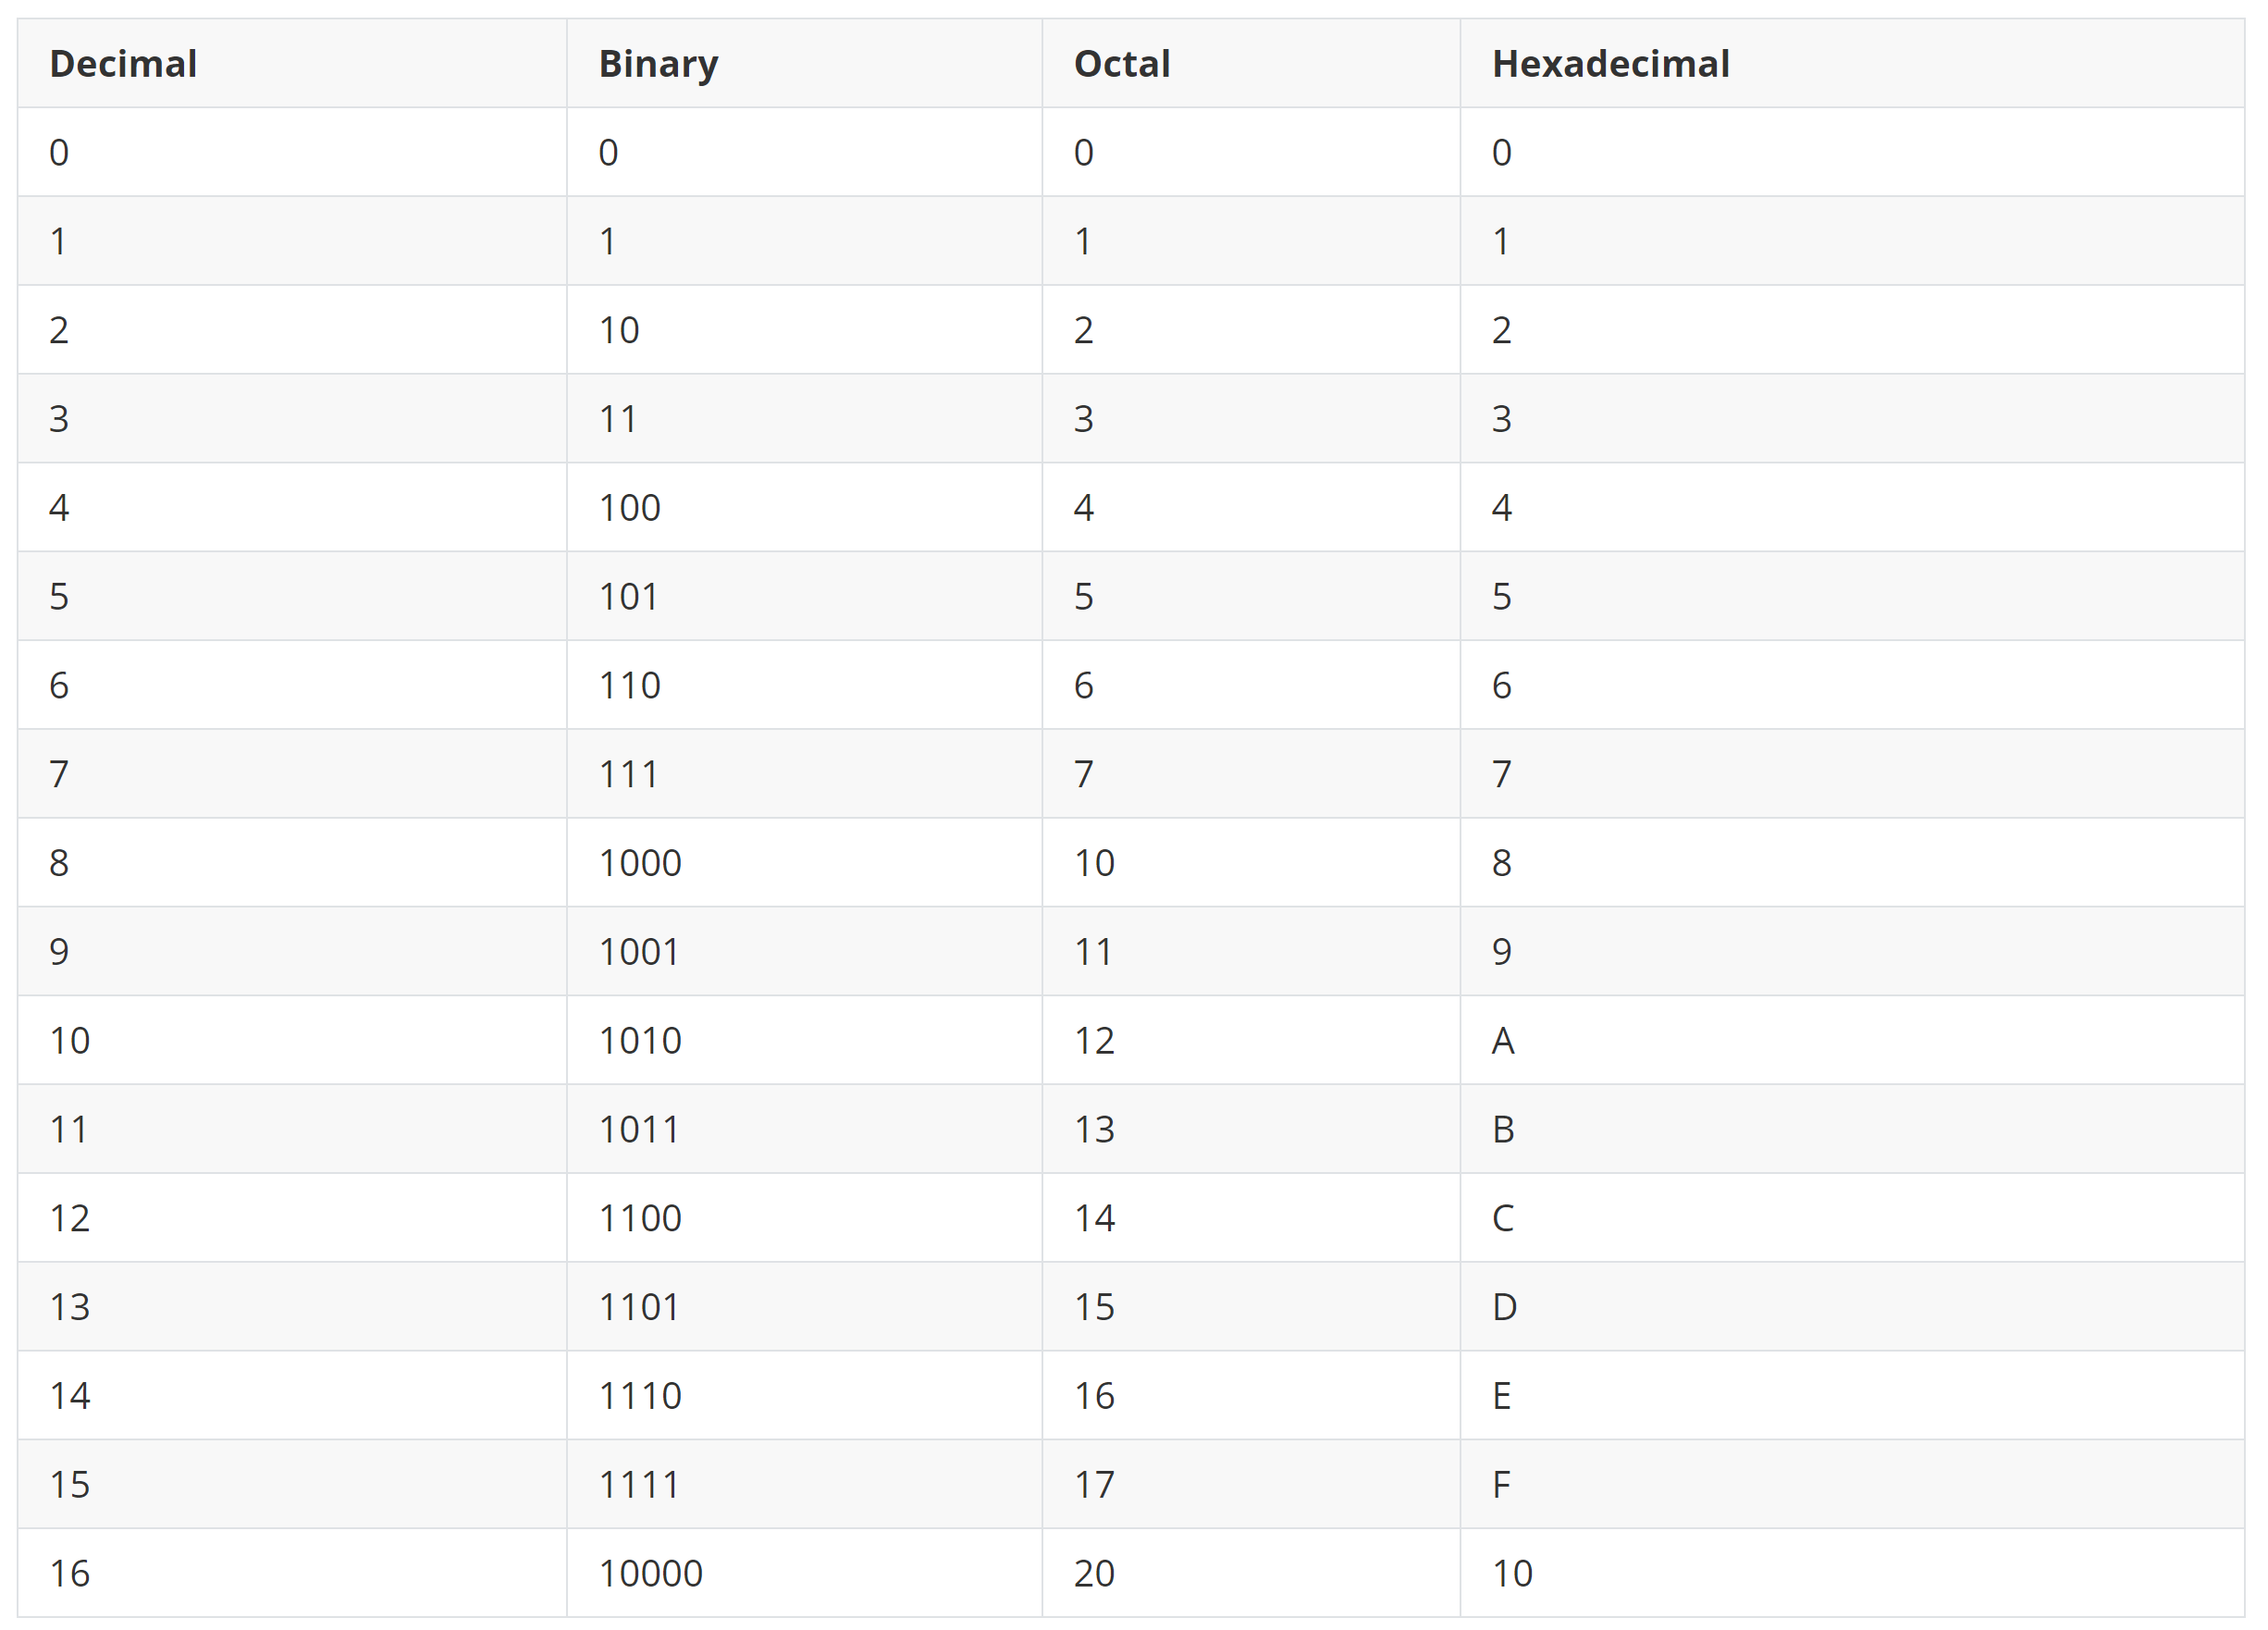
\includegraphics[width=1.2\textwidth]{chapters/ch3/images/Number_Chart.PNG}
\end{center}

\begin{problem}
    Convert $(DB5)_{16}$ into binary and octal.
\end{problem}


\section{Primes and Greatest Common Divsors}

\begin{definition}[Prime Numbers]{def3.3.1:label}
    An integer $p$ greater than 1 is \textbf{prime} if the only positive factors of $p$ are 1 and $p$.
\end{definition}

\begin{theorem}[The Fundamental Theorem of Arithmetic]{theorem3.3.1:label}
    Every integer greater than 1 can be written uniquely as a prime or as the prodct of two or more primes written in increasing order.
\end{theorem}

\begin{problem}
    Fnid the prime factorizations of the following numbers:

    \begin{itemize}
        \item $36 = 6^2 = (2\cdot 3)^2 = 2^2\cdot 3^2$\\
        \item $84 = 7 \cdot 12 = 7 \cdot 3 \cdot 2 \cdot 2 = 2^2\cdot 3 \cdot 7$
        \item $31 = 31 \cdot 1$
    \end{itemize}
\end{problem}

\begin{proposition}{prop3.3.1:label}
    If $n$ has a prime divisor, then it must have one that is less than or equal to $\sqrt{n}$
\end{proposition}

Listed below is a table with all of the primes that are $\le 100$. Every number that is \textbf{bold} is a prime number.

\begin{center}
    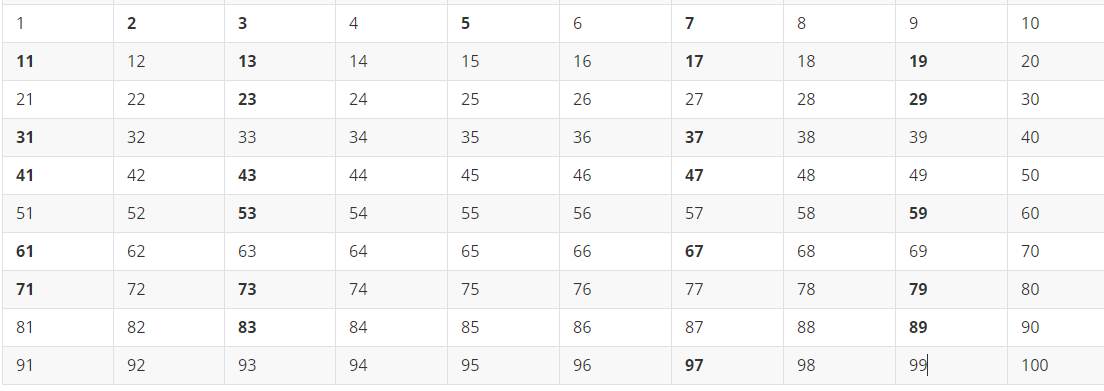
\includegraphics[width=1.2\textwidth]{chapters/ch3/images/Primes_Chart.PNG}
\end{center}


\begin{theorem}{3.3.2:label}
    There are infinietly many primes.
\end{theorem}

\begin{definition}{3.3.2:label}
    Let $a$ and $b$ be integers with $a$ and $b$ not being equal to 0. The largest integer $d$ such that $d|a$ and $d|b$ is called the \textbf{greatest common divisor} of $a$ and $b$. The notation is $\gcd(a,b)$
\end{definition}

\begin{problem}
    Find $\gcd(36,84).$

    $$
    \begin{aligned}
        36 &= 6 \cdot 6 = 2^2 \cdot 3^2\\
        84 &= 7 \cdot 12 = 2^2 cdot 3 \cdot 7\\
        \gcd(36,84) &= 2^2 \cdot 3 = 12
    \end{aligned}
    $$
\end{problem}

\begin{problem}
    Find $\gcd(9,49).$

    $$
    \begin{aligned}
        9 &= 3^2\\
        49 &= 7^2\\
        \gcd(9,49) &= 1
    \end{aligned}
    $$
\end{problem}


\begin{definition}[Relatively Prime]{def3.3.3:label}
    Two integers $a$ and $b$ are \textbf{relatively prime} if $\gcd(a,b) = 1$.
\end{definition}


\begin{definition}{def3.3.4:label}
    The least common multiple of the positive integers $a$ and $b$ is is the smallest positive integer that is divisible by both $a$ and $b$. Notation is $\lcm(a,b)$.
\end{definition}


\chapter{Work, Energy, and Momentum}
\section{Introduction to Work}

\begin{definition}{def4.1:label}
    \textbf{WORK: How much energy it takes to do a certain physical action.}

    $$
    W = \Delta E = \vec F \cdot \vec {\Delta x}
    $$

    $W$ = Work done (SI Units: $\J = \N\m$)\\
    $\Delta E$ = Change in energy\\
    $\vec F$ = the force applied\\
    $\Delta x$ = the displacement over which the object was applied the given force $\vec F$
\end{definition}


\begin{problem}
    A couch is pushed with a force 25 $\N$ over a distance of 5 $\m$. Calculate the work that is applied to the couch. 

    $$
    \begin{aligned}
        W &= F_A \cdot \Delta x\\
        W &= (25 \N)(5 \m)\\
        W &= 100 \J
    \end{aligned}
    $$
\end{problem}


\begin{problem}
    \textbf{SEE ATTACHED FIGURE}

    a) How much energy is expended by the applied force to move the couch 5 $\m$?
    b) How much energy does the frictional force expend to move the couch 5 $\m$?

    To solve part a):
    $$
    \begin{aligned}
        W_A &= F_{Ax} \cdot \Delta x\\
        W_A &= F\cos\theta \cdot \Delta x\\
        W_A &= (50 \N)\cos(25^\circ)(5 \m)\\
        W_A &= 227 \J
    \end{aligned}
    $$

    To solve part b):
    $$
    \begin{aligned}
        W_f &= -F_f \cdot \Delta x\\
        W_f &= -\mu_kF_N \cdot \Delta x\\
        W_f &= -\mu_k(mg + F_A\sin\theta) \cdot \Delta x\\
        W_f &= -(0.15)((20\kg)(9.81\frac{\m}{\s^2}) + (50\N)\sin(25^\circ))
        W_f &= VALUE
    \end{aligned}
    $$
\end{problem}


\section{Energy}

Energy comes in many different forms. The main forms of energy (as well as the proofs to get their respective equations) are listed below:


\begin{definition}[Kinetic Energy]{def4.2:label}
    If an object is moving, the energy that the object expends is equal to the \textbf{kinetic energy}. 

    $$
    KE = \frac{1}{2}mv^2
    $$

    $KE$ = the kinetic energy expended\\
    $m$ = mass of the object\\
    $v$ = velocity of the object at the given moment where you wish to find the energy
\end{definition}

\begin{proof}
    PROOF OF KINETIC ENERGY HERE
\end{proof}


\begin{definition}[Potential Energy]{def4.3:label}
    $$
    PE = mgh
    $$
\end{definition}

\begin{proof}
    PROOF OF POTENTIAL ENERGY HERE
\end{proof}

\begin{definition}[Spring Energy]{def4.4:label}
    $$
    SE = \frac{1}{2}kx^2
    $$
\end{definition}

\begin{proof}
    PROOF OF SPRING ENERGY HERE
\end{proof}

\textbf{NOTE:} Energy is \textit{positive} if energy is being stored and \textit{negative} if energy is being released.

\subsection{The Usefulness of Energy and Work}

While we have an equation for the work if we know the applied forces, if we know other elements about the system (how fast ) [FINISH THIS LATER]


\begin{problem}
    ADD PROBLEM TEXT LATER

    \begin{center}
        \includegraphics[width=0.5\textwidth]{chapters/ch4/images/fig4_5.PNG}
    \end{center}

    While this problem could be solved using kinematics and Newton's second law, we can also use the Work-Energy theorem. 

    $$
    \begin{aligned}
        W_{in} &= \Delta KE + \Delta PE\\
        F_T \cdot L &= \frac{1}{2}m(v_f - v_i)^2 + mg(h_f - h_i)\\
        F_T \cdot L &= \frac{1}{2}mv_f^2 + mgh_f\\
        v_f &= \sqrt{\frac{2(F_TL - mgh_f)}{m}}\\
        v_f &= \sqrt{\frac{2(F_TL - mg(L\sin\theta))}{m}}
    \end{aligned}
    $$
\end{problem}

\begin{problem}
    A skiier starts at the top of a mountain and is attached a spring at the bottom of the cliff. The skiier will also experience friction for 15m at the bottom of the slope right before the spring. How far was the spring compressed when the skiier reaches the bottom of the slope?

    \begin{center}
        \includegraphics[width=0.5\textwidth]{chapters/ch4/images/fig4_6.PNG}
    \end{center}

    $$
    \begin{aligned}
        W_{in} = 0 &= \Delta PE + \Delta E_s + \Delta E_{T}\\
        0 &= mg(h_f-h_i) + \frac{1}{2}k(x_f-x_i)^2 + \mu_kmgD\\
        0 &= -mgh_i + \frac{1}{2}kx_f^2 + \mu_kmgD\\
        x_f &= \sqrt{\frac{(mgh_i-\mu_kmgD)^2}{k}}\\
        x_f &= \sqrt{\frac{((70\kg)(9.81\frac{\m}{\s^2})(50\m)-(0.15)(70\kg)(9.81\frac{\m}{\s^2})(15\m))^2}{150 \frac{\N}{\m}}}\\
    \end{aligned}
    $$
\end{problem}


\begin{problem}
    A stunt artist was launched out of a cannon on a 20m pedestal. He will land in a bucket attached to a pulley. The pulley also has a 50kg mass attached to it, and the bucket is 10m above the ground. Assume the bucket has no mass and the pulley exerts no friction on the string wrapped around the pulley. What is the speed of the stunt artist right when he lands in the bucket? 
    
    \begin{center}
        \includegraphics[width=0.5\textwidth]{chapters/ch4/images/fig4_7.PNG}
    \end{center}

    $$
    \begin{aligned}
        W = 0 &= \Delta KE_1 + \Delta PE_1 + \Delta KE_2 + \Delta PE_2\\
        0 &= \frac{1}{2}m(v_{f1}-v_{i1})^2 + \frac{1}{2}m_2(v_{f2}-v_{i2})^2 + m_1g(H_{f1} - H_{i1}) + m_2g(H_{f2} - H_{i2})\\
    \end{aligned}
    $$

    ANSWER: $41.3 \frac{\m}{\s}$
\end{problem}


\section{Work and Calculus}

\begin{itemize}
    \item Sometimes, the force being applied to an object over a given distance is variable
    \item If you are given an equation for what the force is (dependent on distance), then $W = \int_{x_i}^{x_f} F(x) dx$
\end{itemize}


\begin{problem}
    If the force applied to an object (as a function of distance) is $F(x) = 5 - 2x$, what is the work done on the object if the object moves 3 \m?

    $$
    \begin{aligned}
        W &= \int_{x_i}^{x_f} F(x) \: dx\\
        W &= \int_{0}^{3} 5-2x \: dx\\
        W &= (5-2(3))-(5-2(0)) = -1-5
        W &= -6 \J
    \end{aligned}
    $$
\end{problem}


\section{Power}

\begin{definition}[Power]{def4.5:label}
    \textbf{Power:} How much energy is expended over a given time interval.

    $$
    P = \frac{\Delta E}{\Delta t} = \frac{W}{t}
    $$

    \textbf{SI Units:} Watts (W)
\end{definition}


\begin{definition}[Instantaneous Power]{def4.6:label}
    If power is rewritten as a function of time $P(t)$, then:

    $$
    E = \int_{t_1}^{t_2} P(t)dt 
    $$

    Likewise, if you want to find the instantaneous power, then:

    $$
    P(t) = \frac{dE}{dt}
    $$
\end{definition}


\begin{problem}
    A block of mass 1000 kg is attached to a pulley at the top of a building. The pulley is attached to a motor that uses 200 kW. What is the final velocity of the block the moment it reaches the top of the building?

    \begin{center}
        \includegraphics[width=0.5\textwidth]{chapters/ch4/images/fig4_8}
    \end{center}

    $$
    \begin{aligned}
        P &= \frac{\Delta E}{\Delta t}\\
        P &= \frac{\Delta KE + \Delta PE}{\Delta t}\\
        P &= \frac{\frac{1}{2}mv^2+mgh}{\Delta t}\\
        v_f &= \sqrt{\frac{2(-mgh+\Delta T P)}{m}}
    \end{aligned}
    $$
\end{problem}


\begin{problem}
    A truck drives up a ramp with an angle of inclination of $15^\circ$. If the truck drives 200 meters in 20 seconds, what is the power of the truck (in kW) after the truck has moved 200 meters? Assume that 10\% of the total energy is lost to the environment.

    $$
    \begin{aligned}
        P &= \frac{\Delta E}{t}\\
        P &= \frac{\Delta KE + \Delta PE}{t}+ 10\%\text{ energy}\\
        P &= \frac{\frac{1}{2}mv^2 + mgh}{t} + 10\%\text{ energy}\\
        P &= \left[\frac{\frac{1}{2}m\left(\frac{\Delta x}{t}\right)^2 + mgL\sin\theta}{t}\right]\frac{1}{0.9}\\
        P &= 98.3 \text{ kW}
    \end{aligned}
    $$
\end{problem}


\begin{problem}
    A person with mass 80 kg is on a scooter on top of a hill that is 30 m tall. The person is pushed off by a spring with a spring coefficient of 1500 N/m. The spring is compressed 2.5 m. The person will then go down a hill and launch into the air, then land in a pit of tar with a coefficient of kinetic friction of 0.8. \\

    a) Find the velocity of the person right after the spring pushes him off.\\

    b) Find the distance the person will travel after he lands in the tar. 

    \begin{center}
        \includegraphics[width=0.75\textwidth]{chapters/ch4/images/fig4_10.PNG}
    \end{center}

    a)

    $$
    \begin{aligned}
        W &= \Delta KE + \Delta E_s\\
        0 &= \frac{1}{2}mv_i^2+\frac{1}{2}k(-x_i)^2\\
        v_i = \sqrt{\frac{kx_i^2}{m}}\\
        v_i = 10.8 \frac{\m}{\s}
    \end{aligned}
    $$

    b)
    $$
    \begin{aligned}
        W &= -\frac{1}{2}m(v_i)^2 + mg(-h_i) + F_fd\\
        0 &= -\frac{1}{2}mv_i^2 + - mgh_i + \mu_kF_Nd\\
        d &= \frac{mgh_i + \frac{1}{2}mv_i^2}{\mu_kmg}\\
        d &= 44.9 \m
    \end{aligned}
    $$
\end{problem}


\begin{problem}
    A ball with mass 2 kg is placed inside a cannon that is launched using a spring with spring constant 200 N/m. The spring is compressed 2 m and is compressed all the way to the ground (so that $PE_i = 0$). The cannon is at an angle of $20^\circ$. What is the maximum height that the ball is launched?

    \begin{center}
        \includegraphics[width=0.75\textwidth]{chapters/ch4/images/fig4_11.PNG}
    \end{center}

    We first need the velocity right when the ball leaves the spring. We can set up a mini Work-Energy problem:
    $$
    \begin{aligned}
        W &= \Delta KE + \Delta PE + \Delta E_s\\
        0 &= \frac{1}{2}mv_i^2 + mgL\sin\theta + \frac{1}{2}k(-(L^2))\\
        \frac{1}{2}mv_i^2 &= \frac{1}{2}kL^2 - mgl\sin\theta\\
        v_i &= \sqrt{\frac{2\left(\frac{1}{2}kL^2 - mgl\sin\theta\right)}{m}}
    \end{aligned}
    $$


    Now we can use the x-component of that velocity to get the final velocity in the overall Work-Energy problem.
    $$
    \begin{aligned}
        W &= \Delta KE + \Delta PE + \Delta E_s\\
        0 &= \frac{1}{2}mv_x^2 + mgh_f + \frac{1}{2}k(-(x^2))\\
        mgh_f &= \frac{1}{2}mv_x^2 -\frac{1}{2}kx^2\\
        h_f &= \frac{\frac{1}{2}mv_x^2 -\frac{1}{2}kx^2}{mg}
    \end{aligned}
    $$
\end{problem}


\section{Non-Conservative Energy}

Not all energy is conserved and remained in the system - sometimes the energy is lost to the environment as thermal energy and sound energy


\begin{problem}
    A skiier skiis down a ramp in two parts. On the first part, the angle of elevation is $30^\circ$ and the kinetic coefficient of friction is 0.2. Once the skiier reaches the bottom of the slope, the new coefficient of kinetic friction is 0.3. The slope is 70m tall.\\

    a) What is the velocity of the skiier at the bottom of the slope?\\

    b) What is the acceleration of the skiier while he is on the slope?\\

    c) What is the distance the skiier will slide once he hits the bottom of the slope?\\

    To solve part a):
    $$
    \begin{aligned}
        W &= \Delta KE + \Delta PE + \Delta E_s + E_{TH}\\
        0 &= \frac{1}{2}m(v_f^2-0) + mg(0-h_i) + F_f\cdot\frac{h_i}{\sin\theta}\\
        v_f^2 &= 2\left(gh_i - g\cos\theta\mu_k\frac{h_i}{\sin\theta}\right)\\
        v_f &= \sqrt{2\left(gh_i - g\cos\theta\mu_k\frac{h_i}{\sin\theta}\right)}\\
        v_f &= \sqrt{2gh_i\left(1 - \frac{\mu_k}{\tan\theta}\right)}\\
        v_f &= 36.374 \frac{\m}{\s}
    \end{aligned}
    $$

    To solve part b):
    $$
    \begin{aligned}
        v_f^2 = v_i^2 + 2aL\\
        a = \frac{v_f^2}{2L}\\
        a = \frac{\m}{\s^2}
    \end{aligned}
    $$

    To solve part c):
    $$
    \begin{aligned}
        W &= \Delta KE + \Delta PE + \Delta E_s + E_{TH}\\
        0 &= \frac{1}{2}m(-v_i^2)+F_fD\\
        D &= \frac{v_i^2}{2\mu_kg}\\
        D &= 240.619\m
    \end{aligned}
    $$
\end{problem}


\begin{problem}
    A rock with mass 10kg falls 5m onto a spring with spring constant 100 N/m. What is the the distance that the spring compresses due to the rock falling onto the spring?\\
    
    INCLUDE FIGURE HERE\\

    $$
    \begin{aligned}
        W &= \Delta KE + \Delta PE + \Delta E_s + E_{TH}\\
        0 &= \Delta PE + \Delta E_s\\
        0 &= mg(0-(h+y))+\frac{1}{2}k(y^2-0)\\
        \text{FINISH THIS PROBLEM LATER}
    \end{aligned}
    $$
\end{problem}


\begin{problem}
    INSERT TEXT ABOUT THE PROBLEM HERE

    \begin{center}
        \includegraphics[width=0.75\textwidth]{chapters/ch4/images/fig4_13.PNG}
    \end{center}

    $$
    \begin{aligned}
        W &= \Delta KE + \Delta PE +\Delta E_s + E_{TH}\\
        E_{TH} &= W - \Delta KE - \Delta PE\\
        E_{TH} &= Pt - \Delta KE - \Delta PE\\
        E_{TH} &= Pt - \frac{1}{2}mv_f^2 - mgd\sin\theta
    \end{aligned}
    $$
\end{problem}



\section{Center of Mass}

\begin{itemize}
    \item A lot of times we are looking at an entire system with a bunch of different objects spread throughout
    \item If this is the case, we want to know where all of the mass for every single object (on average) is concentrated
    \item Finding the point where most of the mass is cnocentrated is called the \textbf{center of mass}
\end{itemize}

\begin{definition}[Center of Mass (1D)]{def4.6.1:label}
    If there are multiple masses $m_1,m_2\dots,m_n$ that are all in 1D space, then the center of mass can be determined using the following equation:

    \[
        m_{c} = \frac{\sum_{i=0}^n m_ix_i}{\sum_{i=0}^n m_i}    
    \]

    Where $x_i$ is the position value for the indicated mass.
\end{definition}


\newpage
\begin{definition}[Center of Mass (2D)]{def4.6.2:label}
    If there are multiple masses $m_1,m_2\dots,m_n$ that are all in 2D space, then the center of mass can be determined using the following equations:

    \[
        \begin{aligned}
            m_{xc} &= \frac{\sum_{i=0}^n m_ix_i}{\sum_{i=0}^n m_i}\\
            m_{yc} &= \frac{\sum_{i=0}^n m_iy_i}{\sum_{i=0}^n m_i} 
        \end{aligned}   
    \]

    Where $x_i$ is the x-position of the indicated mass and $y_i$ is the y-position of the indicated mass.
\end{definition}


\section{Introduction to Momentum}

\begin{definition}[Momentum]{def4.7.1:label}
    \[
    \vec p = m \vec v  
    \]

    \textbf{momentum} is a vector (it's simply a scaled version of velocity) and the SI units are $\kg \frac{\m}{\s}$.
\end{definition}

\begin{itemize}
    \item linear momentum is \textbf{always conserved}
    \item kinetic energy is only conserved in an \textbf{elastic collision}
    \begin{itemize}
        \item \textit{ELASTIC COLLISION}: Where two bodies bounce off of each other
        \item \textit{INELASTIC COLLISION:} When two bodies stick together after the collision
    \end{itemize}
    \item FUN FACT: We can get Newton's second law through differentiating the definition of momentum because $\frac{d}{dt}p = \frac{d}{dt}(mv) \implies F_{net} = ma$
\end{itemize}

\begin{definition}[Impulse]{def4.7.2:label}
    \[
    \vec J = \vec Ft = \Delta \vec p = m(\vec v_f - \vec v_i)
    \]

    \textbf{impulse} is how much is applied to an object over a given period of time
\end{definition}

\begin{itemize}
    \item NOTE: Impulse is the \textbf{area under a Force vs time graph}
\end{itemize}


\begin{problem}
    If a baseball comes in to the left at $50 \frac{\m}{\s}$ and gets hit back to the right with a velocity of $80 \frac{\m}{\s}$ at an angle of $30^\circ$. If the right direction is positive, what is the time interval during which the collision of the ball occurred?

    \[
    \begin{aligned}
        F_{avg}t &= m(v_f-v_i)\\
        F_{avg} &= \frac{m(v_f-v_i)}{t}\\
        F_{avg} &= \frac{m<v_{fx} - v_{ix}, v_{fy}-v_{iy}>}{t}\\
        F_{avg} &= 328.6 \vec i + 80 \vec j = 251.6 \angle 18.5^\circ
    \end{aligned}    
    \]
\end{problem}


\begin{problem}
    A cue ball comes and towards the 6-ball with a speed of $2 \frac{\m}{\s}$. The 6-ball goes down at an angle of $30^\circ$ with a velocity magnitude of $3 \frac{\m}{\s}$. What is the final velocity of the cue ball after the collision?
    
    \[
    \begin{aligned}
        \vec p_i &= \vec p_f\\
        m\vec v_{ci} &= m\vec v_{cf} + m\vec v_6\\
        v_{cf} &= v_{ci}-v_6\\
        v_{cf} &= 2\vec i - (2.6 \vec i - 1.5 \vec j)\\
        v_{cf} &= -0.6\vec i + 1.5 \vec j\\
        v_{Cf} &= 1.62 \angle 62.5^\circ \frac{\m}{\s}
    \end{aligned}  
    \]

    NOTE: You can also choose to solve for the momentums in each direction independently (so say that $p_{xi} = p_{xf}$ and then also $p_{yi} = p_{yf}$ and then solve both individually).
\end{problem}


\chapter{Rotational Kinematics, Torque, and Angular Momentum}
\section{Rotational Kinematics}

\begin{itemize}
    \item While objects can move in a straight line, objects can ALSO move in a circle
    \begin{itemize}
        \item Either an object is orbiting some point or something spins around some center
    \end{itemize}
    
    \item Instead of having position, velocity, and acceleration, we will have \textit{new} terms for moving in a circle instead
    \begin{itemize}
        \item \textbf{Angular position ($\theta$):} How much the object has rotated around the positive $x$-axis
        \item \textbf{Angular velocity ($\omega$):} How fast an object is going in a given direction at any point in the circle
        \begin{itemize}
            \item $\frac{d\theta}{dt} = \omega(t)$
            \item $\theta(t) = \int \omega \: dt$
        \end{itemize}
        \item \textbf{Angular acceleration ($\alpha$):} How fast an object changes it's velocity at any point in the circle of motion
        \begin{itemize}
            \item $\frac{d\omega}{dt} = \alpha(t)$
            \item $\omega(t) = \int \alpha \: dt$
        \end{itemize}
    \end{itemize}

    \item the kinematics equations from translational (standard) motion are the EXACT SAME equations in rotational kinematics, but we simply use the rotational kinematics variables instead of the translational kinematics variables
    
    \newpage
    \begin{definition}[Rotational Kinematics Equations]{def5.1.1:label}
        To calculate different values of 

        \[
        \begin{aligned}
            \omega_f &= \omega_i + \alpha t\\
            \Delta\theta &= \omega_it + \frac{1}{2}\alpha t^2\\
            \omega_f^2 &= \omega_i^2 + 2\alpha\Delta\theta
        \end{aligned}    
        \]
    \end{definition}

    \item it is important to note that values are \textbf{positive} if things move \textit{in the counterclockwise direction} and values are \textbf{negative} if things move \textit{in the clockwise direction}
    \item If you know the distance between the object moving in rotation and the center of rotation (in other words: the radius of the circle of rotation), then you can relate the rotational kinematics values with the translational kinematics values
    
    \begin{definition}[Rotational Kinematics $\leftrightarrow$ Translational Kinematics]{def5.1.2:label}
        \[
        S = \Delta\theta R    
        \]

        Where $S$ is the arc that the object travels around through a given angle $\theta$ and $R$ is the radius (the distance between the object and the center of rotation).

        \[
        v = \omega R    
        \]

        Where $R$ is the radius (the distance between the object and the center of rotation).

        \[
        a_{tangential} = \alpha R    
        \]

        Where $R$ is the radius (the distance between the object and the center of rotation). Note that this is the acceleration that is PENPENDICULAR to the acceleration that points towards the center of the circle.

        \[
        a_{centripetal} = \frac{v^2}{R} = \frac{\omega^2 R^2}{R} = \omega^2 R    
        \]

        Where $R$ is the radius (the distance between the object and the center of rotation). Note that this is the acceleration that points towards the CENTER of the circle. 
    \end{definition}
\end{itemize}


\begin{problem}
    A grinder rotates at 850RPM. Once the grinder turns off, it stops 3 minutes later. What is the angular acceleration and what is the final anglular position of the grinder?\\

    First, convert RPM to radians/second:

    \[
    850 \frac{\text{rev}}{\text{min}}\cdot\frac{2\pi \text{ radians}}{1 \text{ rev}}\cdot\frac{1 \text{ minute}}{60 \text{ seconds}} = 28.\bar{3} \frac{\text{radians}}{\s}   
    \]

    Now find angular acceleration:
    \[
    \alpha = \frac{\Delta \omega}{t} = \frac{\omega_f - \omega_i}{t} = \frac{- 28.3 \frac{\rad}{\s}}{60 \s} = -0.49 \frac{\rad}{\s^2}   
    \]

    Now find the final angular position:
    \[
    \begin{aligned}
        \omega_f^2 &= \omega_i^2 + 2\alpha\Delta\theta\\
        \theta_f &= \frac{\omega_f^2 - \omega_i^2}{2\alpha} + \theta_i\\
        \theta_f &= \frac{-(28.\bar{3} \frac{\rad}{\s})^2}{2(-0.49 \frac{\rad}{\s^2})}\\
        \theta_f &= 817.235 \rad
    \end{aligned}    
    \]
\end{problem}


\begin{problem}
    An object rotates and has a function that defines the angluar acceleration to be $\alpha(t) = 5t^3 - 4t$. You know that the initial rotational velocity is 5 $\frac{\rad}{\s}$ and the initial angular position is 2 radians. 

    \[
    \begin{aligned}
        \omega(t) &= \int_0^t \alpha(t)\:dt\\
        \omega(t) &= \int_0^t 5t^3 - 4t \: dt\\
        \omega(t) &= \frac{5}{4}t^4 - 2t^2 + 2
    \end{aligned}    
    \]
\end{problem}


\section{Moment of Inertia}

\textbf{Intertia} is the distribution of mass around the object's center of mass. This term allows us to differentiate between a disk and a chair that are both 5kg because up to this point we have tretaed those two objects as the same object. 


\section{Force, Energy, and Momentum in Rotation}

\begin{itemize}
    \item In the \textbf{linear world}, $KE = \frac{1}{2}mv^2$, but in the \textbf{rotational world} $KE = \frac{1}{2}I\omega^2$
    \item  In the \textbf{linear world}, $F = ma$, but in the \textbf{rotational world} $\tau = I\alpha$
    \begin{itemize}
        \item It shuold be noted that the above is Newton's Second Law just applied to rotation. Individual torques are $\tau_A = F_Ar\sin\theta$ where $r$ is the distance between the center of rotation and the point where the force is applied.
    \end{itemize}
    \item In the \textbf{linear world}, $W = F \cdot d$, but in the \textbf{rotational world} $W = \tau \cdot \theta$
    \item In the \textbf{linear world}, $P = Fv$, but in the \textbf{rotational world} $P = \tau\omega$
    \item In the \textbf{linear world}, $p = mv$, but in the \textbf{rotational world} $L = I\omega$
\end{itemize}

\begin{problem}
    \begin{center}
        \includegraphics[width=0.75\textwidth]{chapters/ch5/images/fig5_1.PNG}
    \end{center}
\end{problem}

\begin{problem}
    \begin{center}
        \includegraphics[width=0.75\textwidth]{chapters/ch5/images/fig5_2.PNG}
    \end{center}
\end{problem}


\section{Smooth Rolling Motion}

\[
\begin{aligned}
    \sum F_x  &= ma_{COM} = F_f\\
    \sum \tau_{NET} &= I\alpha = \tau_{APP} - \tau_f = \tau_{APP} - F_fR
\end{aligned}    
\]



\section{Newton's Second Law for Rotation}

\[
\begin{aligned}
    \tau &= I\alpha\\
    F_fR &= I\alpha\\
\end{aligned}    
\]


\section{Angular Momentum and Impulse}

\begin{itemize}
    \item We've been used to \textit{linear momentum} but there is also \textbf{angular momentum} that functions under the same properties
    
    \begin{definition}[Angular Momentum]{def5.6.1:label}
        \[
        L = I\omega     
        \]

        In every case in this class, \textbf{angular momentum will always be conserved}
    \end{definition}

    \item Angular momentum is the reason that an ice skater changes their speed
    \begin{itemize}
        \item When the skater holds out their arms, then the 
    \end{itemize}
\end{itemize}

\begin{problem}[Merry Go Round]
    \[
    \begin{aligned}
        L_i &= L_f\\
        I_m\omega_i &= I_m\omega_f + I_\parallel\omega_f\\
        \omega_f &= \frac{I_m\omega_i}{I_m + I_\parallel}
    \end{aligned}    
    \]
\end{problem}


\begin{problem}[Merry Go Round with Dog]
    \[
    \begin{aligned}
        L_i &= L_f\\
        I_m\omega_i + I_D\omega_i &= I_m\omega_f + I_D(\omega_f - \omega_D)
    \end{aligned}    
    \]
\end{problem}

\begin{itemize}
    \item Additionally, we can get an angular impulse similarly to how we get a linear impulse
    
    \begin{definition}[Angular Impulse]{def5.6.2:label}
        \[
        J_\angle = \tau_{AVG}\Delta T = I \Delta \omega      
        \]
    \end{definition}
\end{itemize}


\begin{problem}[Grindstone Problem]
    \[
    \begin{aligned}
        L_i &= L_f\\
        I_1\omega_i &= I_1\omega_f + I_2\omega_f\\
        I_1\omega_i &= \omega_f(I_1 + I_2)\\
        \omega_f &= \frac{I_1}{I_1+I_2}\omega_i\\
        \omega_f &= \frac{0.5M_1R_1^2}{0.5M_1R_1^2+0.5M_2R_2^2}\omega_i\\
    \end{aligned}    
    \]
\end{problem}


\chapter{Statics}
\section{Biconditional Statements}

\begin{itemize}
    \item Recall that "$P$ iff $Q$ is equivalent to "If $P$ then $Q$ and if $Q$ then $P$".
    \item If you want to write a biconditional proof, write a proof for if $P$ then $Q$ and then write another proof for if $Q$ then $P$. 
\end{itemize}

\begin{proposition}
    The integer $n$ is odd if and only if $n^2$ is odd. 
\end{proposition}

\begin{proof}
    \subsubsection*{$\implies$}


    \subsubsection{$\implies$}

    Suppose $n$ is even. This means there is some integer $k$ such that $n = 2k$. This means that $n^2 = (2k)^2 = 4k^2 = 2(2k^2)$. Since $k$ is an integer, then $2k^2$ is also an integer. 
\end{proof}


\section{Equivalence Statements}

\begin{itemize}
    \item This is a generalization of biconditional statements
    \item We will use the phrase "the following are equivalent" (TFAE)
\end{itemize}

\begin{theorem}[The Invertible Matrix Theorem]{theorem6.1.1:def}
    Let $A$ be a square matrix. Then the following statements are equivalent:

    \begin{enumerate}
        \item $A$ is invertible
        \item $A$ is row equivalent to the $n\times n$ identity matrix
        \item $A$ has $n$ pivot positions
        \item The equation $A\vec{x} = \vec{0}$ has only the trivial solution
        \item The columns of $A$ form a linearly indepentent set
        \item The linear transformation $\vec \rightarrow A\vec{x}$ is one-to-one
        \item The equation $A\vec{x} = \vec{b}$ has at least one solution for each $\vec{b}$ in $\R^n$
        \item The columns of $A$ span $\R^n$
        \item The linear transformation $\vec{x} \rightarrow A\vec{x}$ maps $\R^n$ onto $R^n$
        \item There is an $n\times n$ matrix $C$ such that $CA = I$
        \item There is an $n\times n$ matrix $D$ such that $AD = I$
        \item $A^T$ is invertible
    \end{enumerate}
\end{theorem}

    \begin{center}
        \includegraphics[width=1\textwidth]{chapters/ch6/images/fig6.1.PNG}
    \end{center}


\section{Existence and Uniqueness}

If you want to prove a statement such as $\exists x, P(x)$ or $\exists ! x, P(x)$, all you have to do is come up with one example that causes the statement to be true. This is the \textit{one} time that we are allowed to prove something by example!\\

There are two different types of proofs that fall under this category:

\begin{itemize}
    \item \textbf{constructive proofs:} Prove that the statement is true by constructing/showing one specific example. 
    \item \textbf{nonconstructive proofs:} show that the statement needs to exist, but you don't (or sometimes can't) give a specific example.
\end{itemize}


\begin{proposition}
    TThere is an even prime.
\end{proposition}

\begin{proof}
    (constructive proof) 2 is an even prime because $2=2\cdot 1$ is the only factorization of 2 which means it is prime, and it is even because it can be written as $2(1)$ which is two times some integer (the form of an even number). 
\end{proof}


\begin{proposition}
    FFor any set of five integers, there is a subset of three integers whose sum is a multiple of 3. 
\end{proposition}

\begin{proof}
    (nonconstructive proof) Let $S = \{a,b,c,d,e\}$, where $a,b,c,d,e\in\Z$. If any three elements of $S$ are equivalent mod 3, then we claim that their sum is divisible by 3. Suppose then that $a\equiv b\equiv c \mod 3$. Then for some $d \in \{0,1,2\}$ and for some $k,l,m\in\Z$, we have that $a=3k+d$, $b=3l+d$, $c=3m+d$. This means that:

    \[
        a+b+c = (3k+d) + (3l+d) + (3m+d) + 3(k+l+m) + 3d  
    \]

    Now, if there are not three equivalent numbers mod 3, it msut be that by the pigeonhole principle, there must be at least one number in each equivalence class mod 3. If, say, $a=3k$, $b=3l+1$, and $c=3m+2$ for some $k,lm\in\Z$, then:

    \[
        a + b + c = 3k + (3l+1) + (3m+2) = 3(k+l+m) + (1+2) = 3(k+l+m+1)  
    \]
\end{proof}


\chapter{Fluids}
\section{General Fluid Statics Terms}

\begin{itemize}
    \item \textbf{FLUID:} A substance that accompanies chips and salsa
    \item \textbf{DENSITY:} $m = \rho V$
    \begin{itemize}
        \item The denisity of water is $\rho_{water} = 1000 \frac{\kg}{\m^3} = 1 \frac{\g}{\cm^3}$
    \end{itemize}
    \item \textbf{COMMON VOLUME UNITS:} Liter, Cubic Meter
    \begin{itemize}
        \item $1 \text{ Liter } = 1000 \text{ cm}^3$
        \item $1000 \text{ Liter } = 1 \text{ m}^3$
    \end{itemize}
    \item \textbf{PRESSURE:} $P = \frac{F}{A_\perp}$
    \begin{itemize}
        \item PRESSURE AT SEA LEVEL: $14.7 \psii = 1.01 \times 10^5 \pa = 101 \text{ KPa}$
    \end{itemize}
\end{itemize}

\begin{problem}[Basic Pressure Problem]
    A room is $3.5\m \times 4.2\m \times 2.4\m$. If the density of air is $1.21 \frac{\kg}{\m^3}$, what is the force weight in the room and the pressure at the floor of the room?

    \[
    \begin{aligned}
        W &= mg\\
        W &= \rho_{air}V_{room}g\\
        W &= (1.21)(3.5)(4.2)(2.4)(9.81)\\
        W &= 418 \N 
    \end{aligned}    
    \]

    \[
    \begin{aligned}
        P &= \frac{F}{A}\\
        P &= \frac{\rho_{air}lwhg}{wl}\\
        P &= \rho_{air}hg\\
        P &= (1.21)(2.4)(9.81)\\
        P &= 28.44 \pa
    \end{aligned}    
    \]
\end{problem}\newpage

\begin{definition}[General Pressure Equations]{def7.1.1:label}
    The pressure at a given reference point $R$ is given by the following equation:

    \[
    \begin{aligned}
        P = P_R \pm \rho Hg
    \end{aligned}    
    \]

    If you want to find the \textbf{absolute pressure} at a point $R$, then you can use the following equation:

    \[
    P = P_{atm} \pm \rho Hg    
    \]

    The \textbf{guage pressure} is the pressure experience without considering atmospheric pressure, which is given by the following equation:

    \[
    \begin{aligned}
        P - P_{atm} = \rho Hg
    \end{aligned}    
    \]
\end{definition}


\begin{problem}
    There is a pipe that is in the shape of a square D without the top. Water is put in the pipe so that the water is at the same height on both sides of the pipe. Oil is placed on the left side of the pipe and the height of the water rises on the right. What is the density of the oil?

    \[
    \begin{aligned}
        P_{atm} + \rho_{oil}gD = P_{atm} + \rho_{water}gy_1\\
        \rho_{oil} = \rho_{water}\frac{y_1}{D}
    \end{aligned}    
    \]
\end{problem}

\begin{itemize}
    \item A force on an imcompressible fluid is additive - that is if you enact a force down on a fluid, you add the created pressure to the reference pressure of the point in the fluid you wish to analyze.
\end{itemize}


\section{Archimedes' Principle}

\begin{definition}[Archimedes' Principle]{def7.2.1:label}
    An object that is submerged in water is equal to the weight of the displaced fluid. The weight of the displaced fluid is called the \textbf{buoyant force}.

    \[
    F_B = V\rho g    
    \]
\end{definition}

\begin{problem}[The Concrete Canoe]
    \[
    \begin{aligned}
        \sum F &= 0 = F_B - mg\\
        F_B &= mg\\
        \rho_{water}V_{disp}g &= \rho_{obj}V_{obj}g
    \end{aligned}    
    \]
\end{problem}


\begin{problem}[The (Floating?) Rock]
    \[
    \begin{aligned}
        \sum F_y &= 0 = F_B + N - W\\
        N &= W - F_B\\
        N &= \rho_RVg - \rho_WVg\\
        N &= Vg(\rho_R-\rho_W)
    \end{aligned}    
    \]
\end{problem}

\begin{problem}[Floating Wood]
    \[
    \begin{aligned}
        \sum F_y &= F_B - W\\
        F_B &= W\\
        \rho_{H_20}(H-y)wlhg &= \rho_Whwlg\\
        \rho_{H_20}H - \rho_{H_20}y &= \rho_Wh\\
        y &= h(\rho_{H_20} - \rho_W)\\
        y &= \frac{H(\rho_{H_20}-\rho_W)}{\rho_{H_20}}
    \end{aligned}    
    \]
\end{problem}

\begin{problem}[Dams (Damn)]
    \[
    \begin{aligned}
        dF &= P(y)W(y)dy\\
        P(y) &= P_r + \rho g y\\
        \int_{F = 0}^{F_{net}}dF &= \int_0^{100}(\rho gy)\left(W-\frac{y}{2}\right)\\
        \rho g \int_0^{100}\left(Wy - \frac{y^2}{2}\right)dy &=
    \end{aligned}     
    \]
\end{problem}


\end{document}
